\section{Phân tích và Thiết kế}
\subsection{Phân tích}
\subsubsection{Mô hình hóa tương tác}

\subsubsubsection{Tổng quan}
\begin{figure}[H]
    \centering
    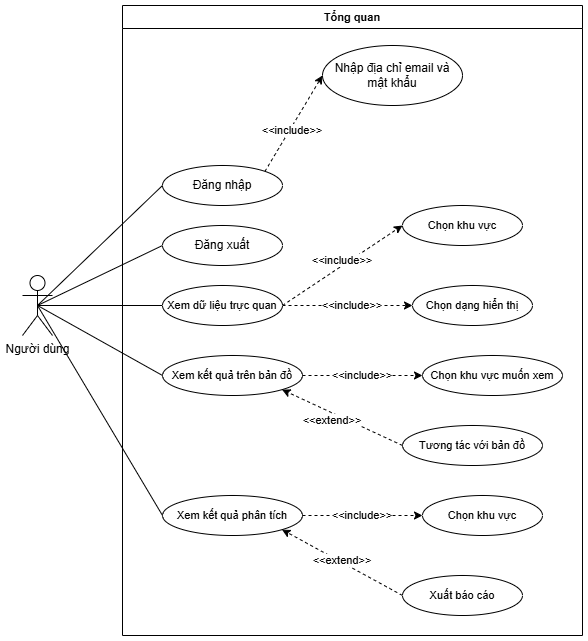
\includegraphics[width=0.9\linewidth]{Images/Usecase tổng quan.drawio.png}
    \caption{Sơ đồ Use Case tổng quan}
\end{figure}

\subsubsubsection{Đăng nhập và đăng xuất}
\begin{figure}[H]
    \centering
    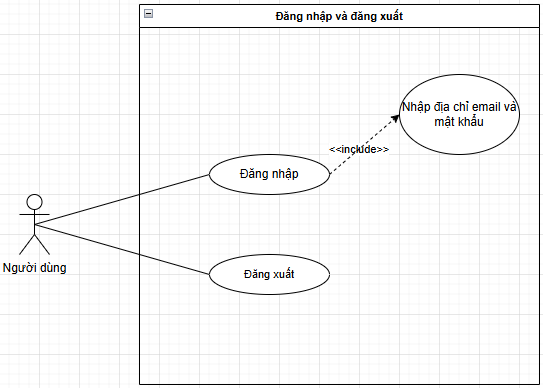
\includegraphics[width=0.9\linewidth]{Images/Usecase1.png}
    \caption{Sơ đồ Use Case đăng nhập và đăng xuất}
\end{figure}
\begin{table}[H]
\centering
\begin{tabular}{|p{0.28\linewidth}|p{0.62\linewidth}|}
\hline
\textbf{Tên use case} & Đăng nhập \\ \hline

\textbf{Mô tả} & 
Cho phép người dùng (đã có tài khoản) truy cập vào hệ thống bằng thông tin xác thực của họ. \\ \hline

\textbf{Tác nhân} & Người dùng (đã có tài khoản). \\ \hline

\textbf{Điều kiện kích hoạt} & 
Người dùng ở trạng thái chưa đăng nhập nhấn vào nút “Đăng nhập”. \\ \hline

\textbf{Điều kiện tiên quyết} &
Người dùng đang ở trạng thái chưa đăng nhập nhưng đã có tài khoản. \\ \hline

\textbf{Điều kiện sau hành động} &
Nếu thành công, người dùng được xác thực và chuyển đến trang tài khoản. Nếu thất bại, hệ thống hiển thị lỗi. \\ \hline

\textbf{Luồng chính} &
1. Người dùng nhấp vào giao diện “Đăng nhập”. \newline
2. Nhập email và mật khẩu. \newline
3. Nhấn “Đăng nhập”. \newline
4. Hệ thống kiểm tra và xác thực thông tin. \newline
5. Hệ thống tạo phiên đăng nhập và chuyển người dùng đến trang chủ. \\ \hline

\textbf{Luồng rẽ nhánh} & 
5a. Email hoặc mật khẩu không chính xác dẫn đến hệ thống báo lỗi và yêu cầu nhập lại. \\ \hline

\textbf{Kết quả} & Phiên đăng nhập được tạo hoặc hiển thị lỗi. \\ \hline
\end{tabular}
\end{table}

\begin{table}[H]
\centering
\begin{tabular}{|p{0.28\linewidth}|p{0.62\linewidth}|}
\hline
\textbf{Tên use case} & Đăng xuất \\ \hline

\textbf{Mô tả} & 
Cho phép người dùng (đã đăng nhập) thoát ra khỏi tài khoản đang đăng nhập. \\ \hline

\textbf{Tác nhân} & Người dùng \\ \hline

\textbf{Điều kiện kích hoạt} &
Người dùng nhấn vào nút “Đăng xuất”. \\ \hline

\textbf{Điều kiện tiên quyết} &
Người dùng đang trong trạng thái đăng nhập. \\ \hline

\textbf{Điều kiện sau hành động} &
Phiên đăng nhập bị hủy và chuyển hướng về trang đăng nhập (trạng thái chưa đăng nhập). \\ \hline

\textbf{Luồng chính} &
1. Người dùng nhấn nút “Đăng xuất”. \newline
2. Hệ thống hủy phiên đăng nhập. \newline
3. Hệ thống xóa thông tin đăng nhập (cookies, local storage nếu có). \newline
4. Chuyển hướng người dùng về trang đăng nhập. \\ \hline

\textbf{Luồng rẽ nhánh} &
Không có. \\ \hline

\textbf{Kết quả} &
Người dùng trở về trạng thái chưa đăng nhập. \\ \hline
\end{tabular}
\end{table}

\subsubsubsection{Trực quan hóa dữ liệu}
\begin{figure}[H]
    \centering
    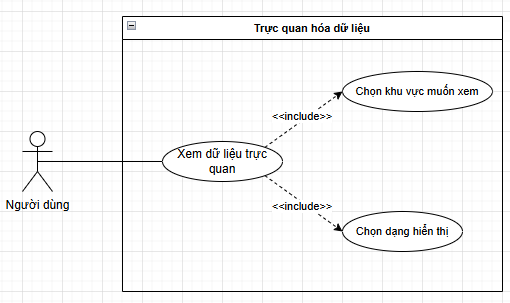
\includegraphics[width=0.9\linewidth]{Images/Usecase2.png}
    \caption{Sơ đồ Use Case trực quan hóa dữ liệu}
\end{figure}
\begin{table}[H]
\centering
\begin{tabular}{|p{0.28\linewidth}|p{0.62\linewidth}|}
\hline
\textbf{Tên use case} & Trực quan hóa dữ liệu \\ \hline

\textbf{Mô tả} & 
Cho phép nhà phân tích quan sát dữ liệu giao thông dưới dạng biểu đồ như: biểu đồ thời gian, biểu đồ phân phối, heatmap, hoặc biểu đồ so sánh nhằm hỗ trợ việc phân tích. \\ \hline

\textbf{Tác nhân} & Người dùng. \\ \hline

\textbf{Điều kiện kích hoạt} & 
Người dùng yêu cầu xem dữ liệu hoặc xem kết quả xử lý dữ liệu ở dạng biểu đồ. \\ \hline

\textbf{Điều kiện tiên quyết} &
Dữ liệu giao thông đã được tiền xử lý và sẵn sàng để hiển thị. \\ \hline

\textbf{Điều kiện sau hành động} &
Biểu đồ hoặc hình ảnh trực quan được tạo và hiển thị để phục vụ phân tích. \\ \hline

\textbf{Luồng chính} &
1. Người dùng chọn khu vực muốn xem (có thể là đoạn đường, phường hoặc quận). \newline
2. Chọn loại biểu đồ muốn hiển thị. \newline
3. Hệ thống xử lý và tạo biểu đồ tương ứng. \newline
4. Biểu đồ được hiển thị cho nhà phân tích xem hoặc lưu lại. \\ \hline

\textbf{Luồng rẽ nhánh} & 
3a. Nếu dữ liệu thiếu hoặc không hợp lệ, hệ thống sẽ hiển thị thông báo lỗi. \\ \hline

\textbf{Kết quả} & Biểu đồ hiển thị thành công hoặc thông báo lỗi nếu dữ liệu không hợp lệ. \\ \hline
\end{tabular}
\end{table}

\subsubsubsection{Hiển thị kết quả phân tích trên bản đồ}
\begin{figure}[H]
    \centering
    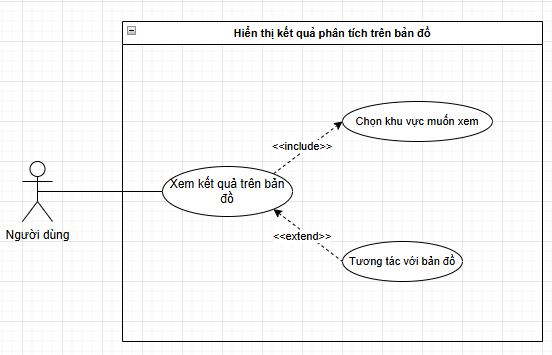
\includegraphics[width=0.9\linewidth]{Images/Usecase3.png}
    \caption{Sơ đồ Use Case hiển thị kết quả phân tích trên bản đồ}
\end{figure}
\begin{table}[H]
\centering
\begin{tabular}{|p{0.28\linewidth}|p{0.62\linewidth}|}
\hline
\textbf{Tên use case} & Hiển thị kết quả phân tích trên bản đồ \\ \hline

\textbf{Mô tả} & 
Cho phép người dùng quan sát kết quả phân tích giao thông trực tiếp trên bản đồ, bao gồm tô màu đoạn đường theo tốc độ, mức độ ùn tắc hoặc các thông số phân tích khác. \\ \hline

\textbf{Tác nhân} & Người dùng. \\ \hline

\textbf{Điều kiện kích hoạt} & 
Người dùng yêu cầu xem kết quả phân tích trên nền bản đồ. \\ \hline

\textbf{Điều kiện tiên quyết} &
Dữ liệu có chứa thông tin không gian (đoạn đường, tọa độ, hoặc dạng network). \\ \hline

\textbf{Điều kiện sau hành động} &
Hiển thị bản đồ với các tuyến đường được tô màu theo giá trị tương ứng; nhà phân tích có thể quan sát và ghi nhận kết quả. \\ \hline

\textbf{Luồng chính} &
1. Người dùng chọn khu vực cần hiển thị. \newline
2. Hệ thống ánh xạ dữ liệu lên bản đồ. \newline
3. Bản đồ được tạo và tô màu theo tốc độ hoặc mức độ ùn tắc. \newline
4. Người dùng tương tác, xem chi tiết hoặc lưu hình ảnh bản đồ. \\ \hline

\textbf{Luồng rẽ nhánh} & 
2a. Thiếu dữ liệu vị trí, hệ thống không thể tạo bản đồ và hiển thị thông báo lỗi. \\ \hline

\textbf{Kết quả} & Bản đồ được hiển thị và sẵn sàng phục vụ phân tích. \\ \hline
\end{tabular}
\end{table}

\subsubsubsection{Xem và xuất báo cáo kết quả phân tích}
\begin{figure}[H]
    \centering
    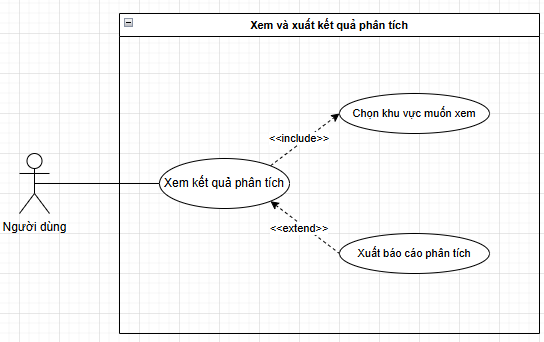
\includegraphics[width=0.9\linewidth]{Images/Usecase4.png}
    \caption{Sơ đồ Use Case xem và xuất kết quả phân tích}
\end{figure}
\begin{table}[H]
\centering
\begin{tabular}{|p{0.28\linewidth}|p{0.62\linewidth}|}
\hline
\textbf{Tên use case} & Xem kết quả phân tích \\ \hline

\textbf{Mô tả} & 
Cho phép người dùng xem các kết quả phân tích tình trạng giao thông, bao gồm các biểu đồ, bản đồ trực quan, thống kê hoặc chỉ số được hệ thống tạo ra từ dữ liệu giao thông đã xử lý. \\ \hline

\textbf{Tác nhân} & Người dùng. \\ \hline

\textbf{Điều kiện kích hoạt} & 
Người dùng truy cập vào mục xem kết quả phân tích hoặc chọn một khu vực để hiển thị kết quả. \\ \hline

\textbf{Điều kiện tiên quyết} &
Hệ thống đã xử lý dữ liệu và tạo ra kết quả phân tích tương ứng. \\ \hline

\textbf{Điều kiện sau hành động} &
Kết quả phân tích được hiển thị dưới dạng biểu đồ, bản đồ hoặc số liệu thống kê. \\ \hline

\textbf{Luồng chính} &
1. Người dùng truy cập chức năng xem kết quả phân tích. \newline
2. Người dùng chọn khu vực muốn xem. \newline
3. Hệ thống truy xuất kết quả phân tích tương ứng từ cơ sở dữ liệu hoặc mô-đun xử lý. \newline
4. Hệ thống hiển thị kết quả dưới dạng biểu đồ, bản đồ hoặc bảng số liệu. \\ \hline

\textbf{Luồng rẽ nhánh} & 
3a. Nếu chưa có kết quả phân tích cho khu vực đã chọn, hệ thống thông báo "Chưa có dữ liệu phân tích". \\ \hline

\textbf{Kết quả} & 
Người dùng xem được kết quả phân tích hoặc nhận thông báo nếu dữ liệu không có sẵn. \\ \hline
\end{tabular}
\end{table}

\begin{table}[H]
\centering
\begin{tabular}{|p{0.28\linewidth}|p{0.62\linewidth}|}
\hline
\textbf{Tên use case} & Xuất báo cáo phân tích \\ \hline

\textbf{Mô tả} & 
Cho phép nhà phân tích xuất các kết quả phân tích (biểu đồ, bảng số liệu, bản đồ, thống kê) thành tệp tin như PDF, CSV hoặc hình ảnh phục vụ trình bày hoặc báo cáo nghiên cứu. \\ \hline

\textbf{Tác nhân} & Người dùng. \\ \hline

\textbf{Điều kiện kích hoạt} & 
Người dùng yêu cầu lưu lại kết quả phân tích dưới dạng tệp. \\ \hline

\textbf{Điều kiện tiên quyết} &
Kết quả phân tích đã được tạo và sẵn sàng để xuất file. \\ \hline

\textbf{Điều kiện sau hành động} &
Hệ thống tạo file báo cáo hoặc hình ảnh và cung cấp cho người dùng để tải xuống. \\ \hline

\textbf{Luồng chính} &
1. Người dùng chọn loại file báo cáo muốn xuất (PDF, CSV, hình ảnh...). \newline
2. Hệ thống tổng hợp dữ liệu và biểu đồ liên quan. \newline
3. Hệ thống tạo tệp báo cáo. \newline
4. Người dùng tải xuống tệp. \\ \hline

\textbf{Luồng rẽ nhánh} & 
2a. Thiếu dữ liệu đầu vào, hệ thống không thể tạo báo cáo và thông báo lỗi. \\ \hline

\textbf{Kết quả} & Tệp báo cáo được tạo thành công hoặc hiển thị lỗi nếu thất bại. \\ \hline
\end{tabular}
\end{table}

\subsubsubsection{Dự báo lan truyền ùn tắc giao thông}

\begin{figure}[H]
    \centering
    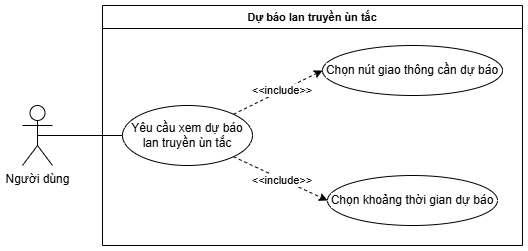
\includegraphics[width=0.9\linewidth]{Images/Usecase5.png}
    \caption{Sơ đồ Use Case dự báo ùn tắc giao thông}
\end{figure}

\begin{table}[H]
\centering
\begin{tabular}{|p{0.28\linewidth}|p{0.62\linewidth}|}
\hline
\textbf{Use case id} & 7 \\ \hline

\textbf{Tên use case} & Dự báo lan truyền ùn tắc giao thông \\ \hline

\textbf{Mô tả} & 
Cho phép người dùng xem dự báo việc một nút giao thông bị tắc nghẽn sẽ ảnh hưởng và lan truyền đến các nút giao thông lân cận nào trong mạng lưới giao thông, đồng thời ước lượng khoảng thời gian lan truyền. \\ \hline

\textbf{Tác nhân} & Người dùng. \\ \hline

\textbf{Điều kiện kích hoạt} & 
Người dùng chọn một nút giao thông đang hoặc có nguy cơ bị tắc nghẽn và yêu cầu hệ thống thực hiện dự báo lan truyền. \\ \hline

\textbf{Điều kiện tiên quyết} &
Dữ liệu giao thông đã được thu thập và tiền xử lý. Mạng lưới giao thông đã được xây dựng. Hệ thống có mô hình hoặc thuật toán dự báo lan truyền ùn tắc.\\ \hline

\textbf{Điều kiện sau hành động} &
Kết quả dự báo được tạo ra, bao gồm danh sách các nút bị ảnh hưởng và thời gian lan truyền tương ứng. \\ \hline

\textbf{Luồng chính} &
1. Người dùng chọn nút giao thông cần dự báo. \newline
2. Người dùng chọn khoảng thời gian dự báo. \newline
3. Hệ thống truy xuất dữ liệu giao thông và cấu trúc mạng lưới liên quan. \newline
4. Hệ thống thực hiện mô phỏng hoặc mô hình dự báo lan truyền ùn tắc. \newline
5. Hệ thống xác định các nút giao thông bị ảnh hưởng và thời gian lan truyền. \newline
6. Kết quả dự báo được hiển thị dưới dạng bản đồ, biểu đồ hoặc bảng số liệu. \\ \hline

\textbf{Luồng rẽ nhánh} &
4a. Nếu dữ liệu không đủ hoặc mô hình không hội tụ, hệ thống hiển thị thông báo lỗi hoặc cảnh báo độ tin cậy thấp. \\ \hline

\textbf{Kết quả} &
Người dùng quan sát được phạm vi lan truyền ùn tắc và thời gian ảnh hưởng, hoặc nhận thông báo nếu dự báo không khả thi. \\ \hline
\end{tabular}
\end{table}

\subsubsection{Mô hình hóa quy trình nghiệp vụ}

\subsubsubsection{Activity diagram}
\begin{figure}[H]
    \centering
    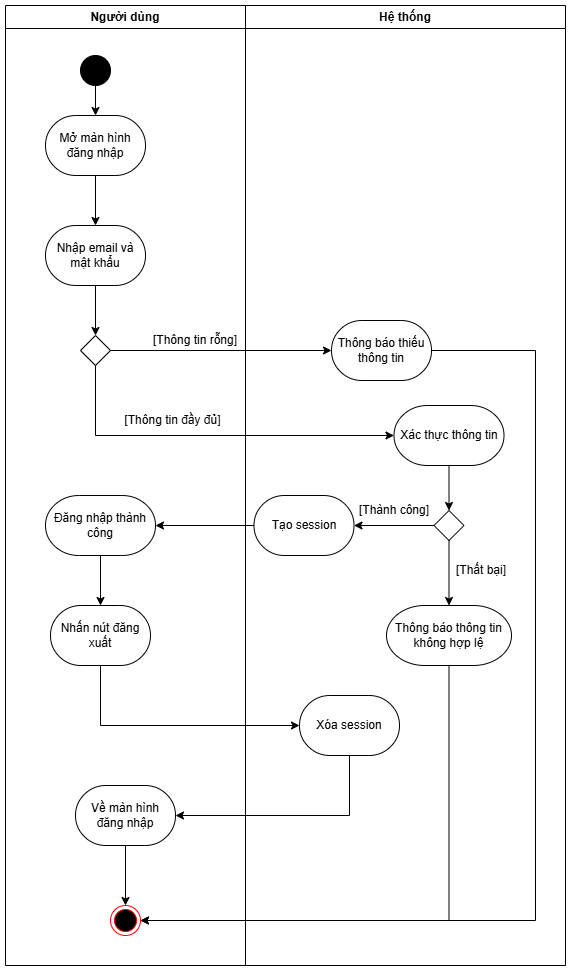
\includegraphics[width=0.7\linewidth]{Images/Act đăng nhập, đăng xuất.png}
    \caption{Sơ đồ Activity đăng nhập, đăng xuất}
\end{figure}

\begin{figure}[H]
    \centering
    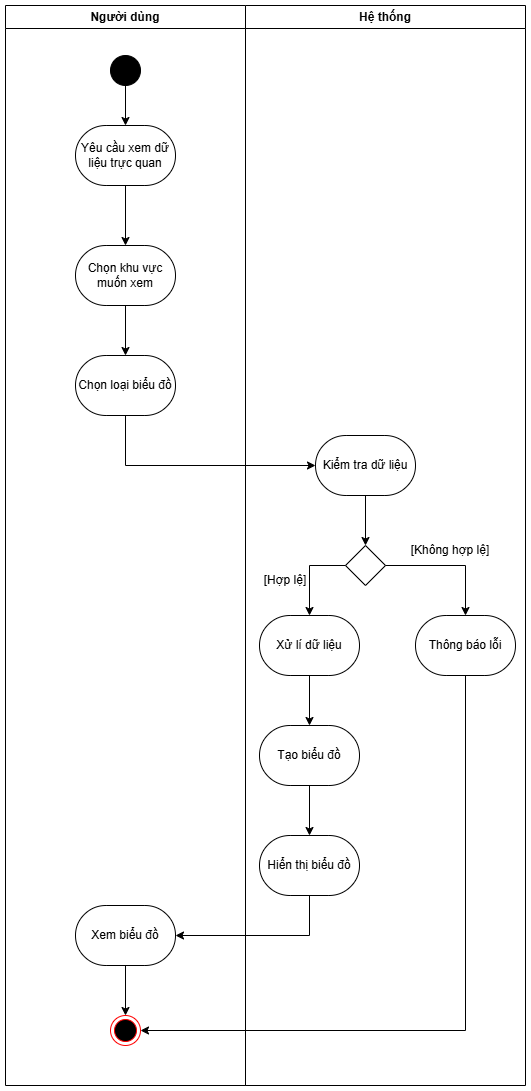
\includegraphics[width=0.7\linewidth]{Images/Act trực quan hóa dữ liệu.png}
    \caption{Sơ đồ Activity trực quan hóa dữ liệu}
\end{figure}

\begin{figure}[H]
    \centering
    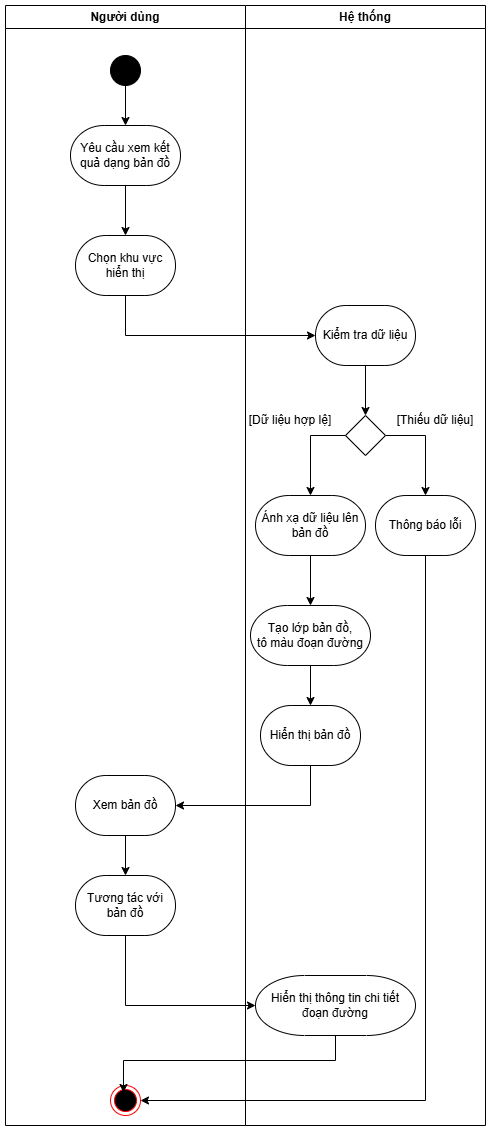
\includegraphics[width=0.6\linewidth]{Images/Act xem kết quả dạng bản đồ.png}
    \caption{Sơ đồ Activity xem kết quả dạng bản đồ}
\end{figure}

\begin{figure}[H]
    \centering
    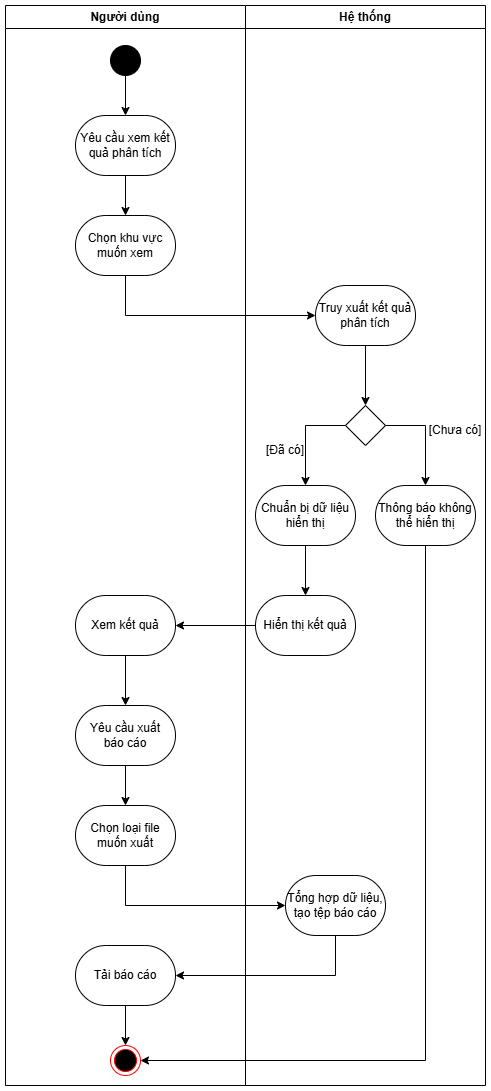
\includegraphics[width=0.6\linewidth]{Images/Act xem và xuất báo cáo.png}
    \caption{Sơ đồ Activity xem và xuất kết quả phân tích}
\end{figure}

\begin{figure}[H]
    \centering
    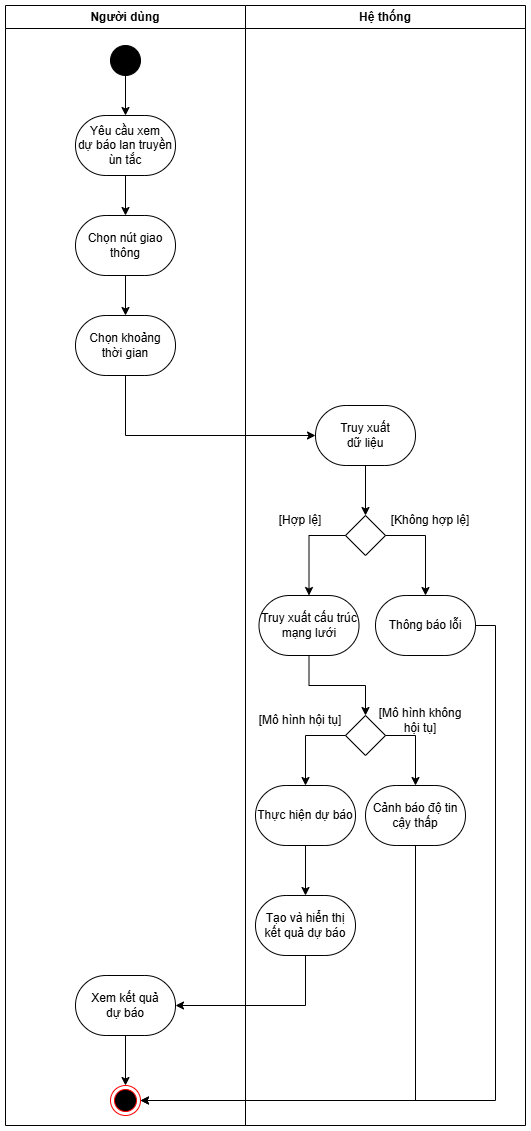
\includegraphics[width=0.7\linewidth]{Images/Act dự báo lan truyền ùn tắc.png}
    \caption{Sơ đồ Activity dự báo lan truyền ùn tắc giao thông}
\end{figure}
\subsubsubsection{Sequence diagram}

\begin{figure}[H]
    \centering
    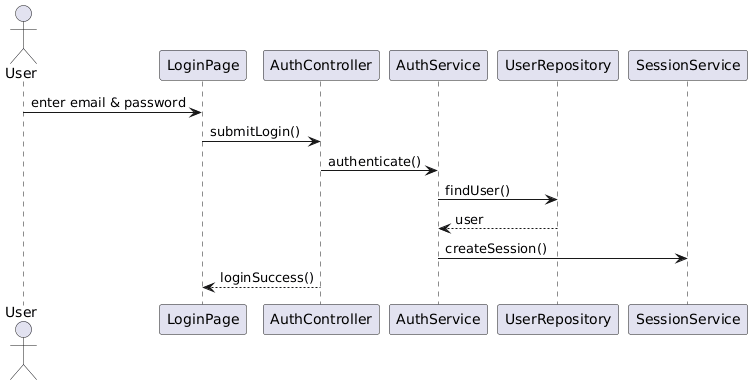
\includegraphics[width=1\linewidth]{Images/Sequence diagram/Login.png}
    \caption{Sơ đồ Sequence đăng nhập}
\end{figure}

\begin{figure}[H]
    \centering
    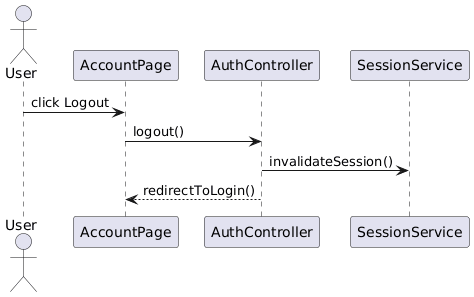
\includegraphics[width=0.9\linewidth]{Images/Sequence diagram/Logout.png}
    \caption{Sơ đồ Sequence đăng xuất}
\end{figure}

\begin{figure}[H]
    \centering
    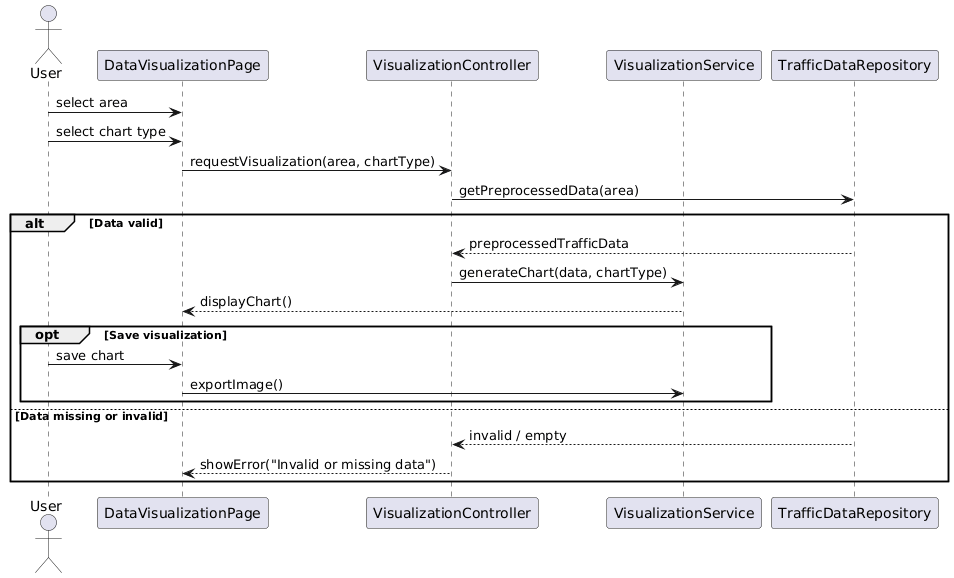
\includegraphics[width=1\linewidth]{Images/Sequence diagram/Visualize Data.png}
    \caption{Sơ đồ Sequence trực quan hóa dữ liệu}
\end{figure}

\begin{figure}[H]
    \centering
    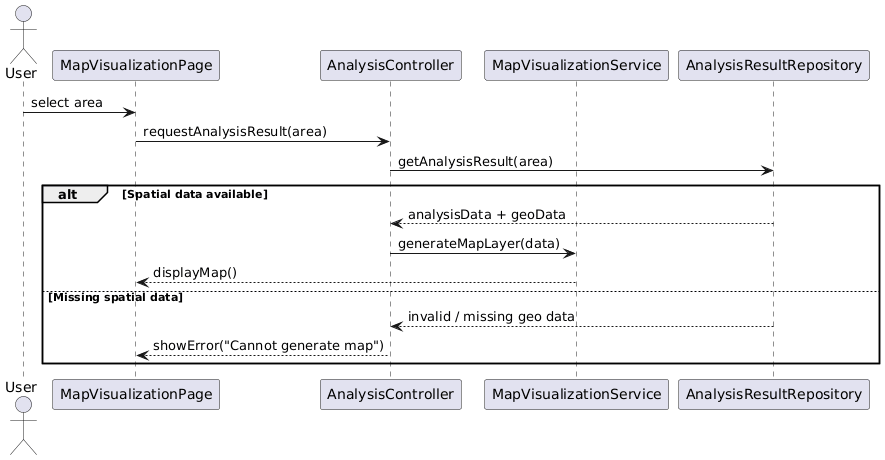
\includegraphics[width=1\linewidth]{Images/Sequence diagram/Analysis Results Map.png}
    \caption{Sơ đồ Sequence xem kết quả dạng bản đồ}
\end{figure}

\begin{figure}[H]
    \centering
    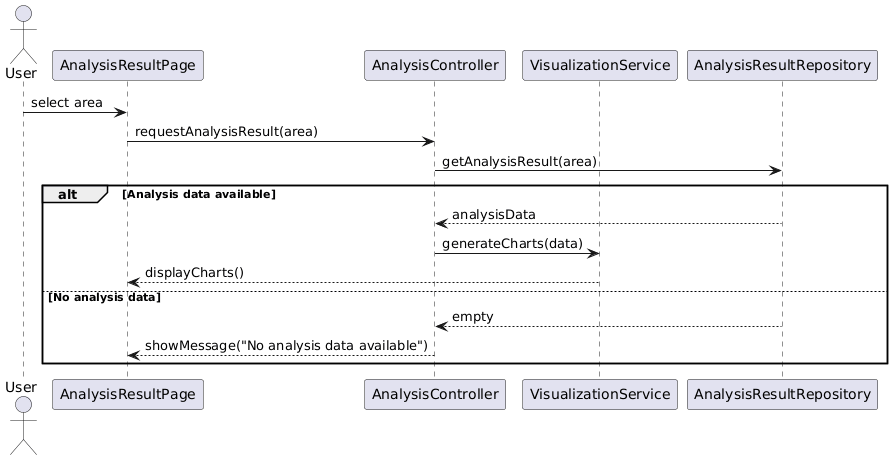
\includegraphics[width=1\linewidth]{Images/Sequence diagram/View Analysis Results.png}
    \caption{Sơ đồ Sequence xem kết quả phân tích}
\end{figure}

\begin{figure}[H]
    \centering
    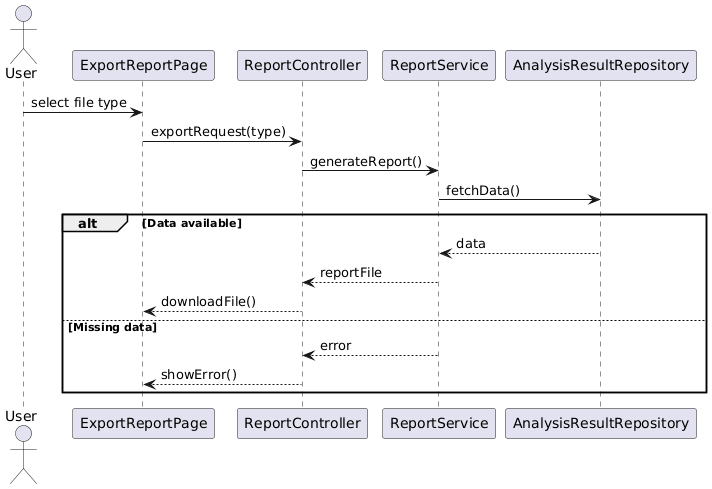
\includegraphics[width=1\linewidth]{Images/Sequence diagram/Export Report.png}
    \caption{Sơ đồ Sequence xuất kết quả phân tích}
\end{figure}

\begin{figure}[H]
    \centering
    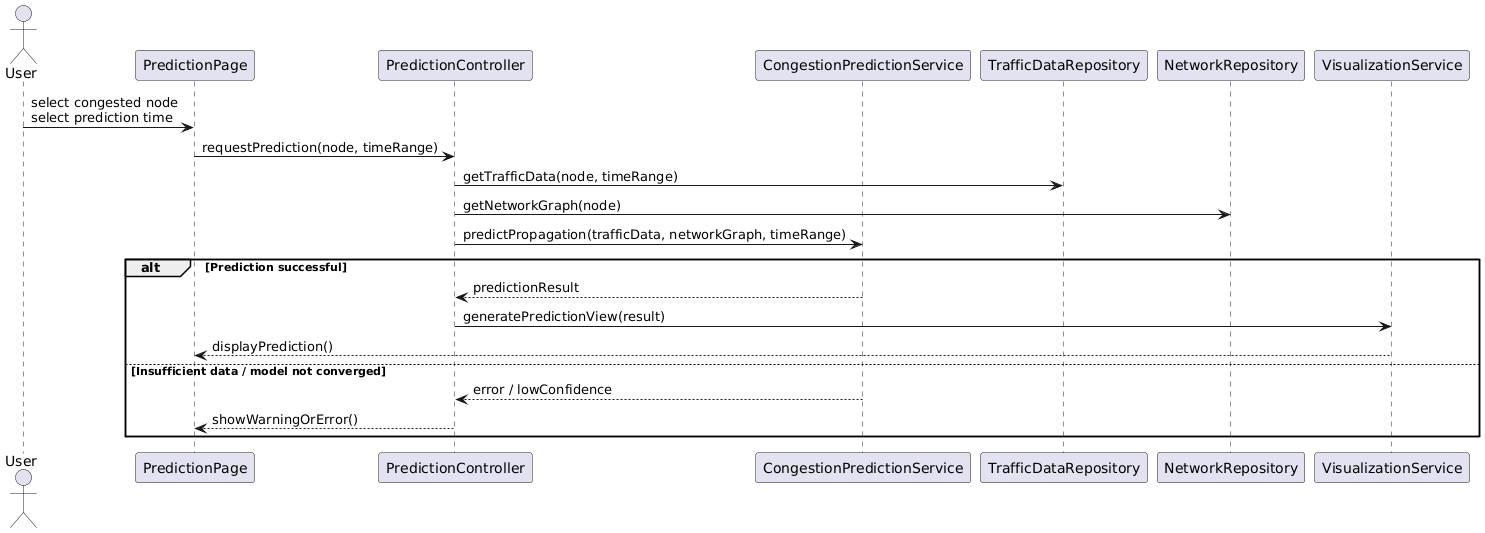
\includegraphics[width=1\linewidth]{Images/Sequence diagram/Predict.png}
    \caption{Sơ đồ Sequence dự báo lan truyền ùn tắc giao thông}
\end{figure}